\documentclass[11pt,a4paper]{article}
\usepackage[utf8]{inputenc}
\usepackage[T1]{fontenc}
\usepackage[margin=19mm]{geometry}
\usepackage{amsmath,graphicx,booktabs,array,longtable,caption}
\usepackage[hidelinks]{hyperref}
\setlength{\tabcolsep}{3pt}
\setlength{\parindent}{0pt}
\setlength{\parskip}{6pt}
\title{Boundary diagnostics, exact-feedback boundaries and the noisy payload comparison in MuJoCo}
\author{Michael Agbo}
\date{12 November 2026}
\begin{document}
\maketitle
\section*{Scope and principal findings}
This supplement answers the two questions left open by the boundary and payload report. First, why do the planar model and the wheel-contact MuJoCo model disagree in exactly two fall-boundary cells? Second, does the reduction in noisy falls from payload-aware LQR redesign, seen so far only in the planar model, persist in the contact model? Both studies are simulations with illustrative parameters. Neither simulator is treated as ground truth, and nothing was fitted to make them agree.

The disagreement has a single sufficient cause. The contact model carries 0.0002 kg m\textsuperscript{2} of chassis pitch inertia that the planar equations omit, 0.39\% of the pitch inertia about the axle. It lowers the contact model's critical push force by 44.6 mN, from 18.2332 N to 18.1887 N. Everything else in the contact model raises its boundary 6.1 mN above the planar 18.2271 N, so the net gap is 38.5 mN (0.21\%), and the 18.2 N grid cell happens to lie inside it. Removing that inertia from the contact model, or adding it to the planar model, exchanges their labels at +18.2 and -18.2 N. The unsettled contact start changes nothing in these cells. Contact and friction settings move the contact model's boundary by -14.0 to +3.1 mN, never enough to change the label, unless friction falls below the traction the manoeuvre needs.

The noisy fall reduction persists in the contact model. With the same loads, disturbances, sensing profiles and noise seeds, fixed LQR falls in 511 of 1,620 trials and payload-aware LQR in 343 at a 0.25 ms physics step (180 falls prevented, 12 introduced), and in 509 and 343 at 0.5 ms (178 prevented, 12 introduced). The archived planar result is 508 and 334 (186 prevented, 12 introduced). A Python port of the sensing pipeline reproduces the outcome of all 3,240 archived planar records before any contact result is used. Every fall, in every plant, occurs at the tighter of the two torque limits, 0.3 N m.

Two analyses added after these results show what the reduction is. With exact state feedback at the same conditions, the redesign changes the fall label in only 2 of the 18 load and scenario conditions. Measured as a boundary, its effect is larger and systematic: it raises the push the robot can withstand without falling by 4\% to 9\% at the 0.26 m mounting height and by 10\% to 21\% at 0.36 m, and lowers it by at most 1.0\% at 0.14 m, with the planar and contact models within 0.04 N of each other. At 0.26 m the 12 N push of the noisy scenario lies just below the fixed gain's boundary (12.17 to 12.93 N), and the noisy fall count of each gain follows its distance to its own boundary, with both gains on one relationship (Spearman rank correlation -0.98 to -0.88 per plant and profile). Noise therefore makes a deterministic boundary shift visible as fewer falls; it does not add a separate benefit. Counted per controller, falls in conditions that the same controller survives without noise number 241 for the fixed gain and 254 for the payload-aware gain in the contact model.

\textbf{Table S1. Study inventory; integrations are not independent experimental samples}
\begin{longtable}{p{0.297\linewidth}p{0.171\linewidth}p{0.126\linewidth}p{0.306\linewidth}}
\toprule
Study & Conditions & Integrations & Result \\ \midrule \endhead
Boundary diagnostics and consistency check & 25 variants, 3 limits & 656 & Chassis inertia explains both cells \\
Noisy payload, planar port & 1,620 pairs & 3,240 & Matches archive in 3,240 of 3,240 outcomes \\
Noisy payload, contact 0.25 ms & 1,620 pairs & 3,240 & 511 to 343 falls \\
Noisy payload, contact 0.5 ms (step check) & 1,620 pairs & 3,240 & 509 to 343 falls \\
Exact-feedback control (post hoc) & 18 conditions, 3 plants & 108 & 2 of 18 fall labels changed, in every plant \\
Exact-feedback boundary (post hoc) & 18 conditions, 3 plants & 2,988 & Boundary raised by up to 21\% \\
Repeatability check & 12 groups & 360 & 360 of 360 records identical \\
\bottomrule
\end{longtable}
\clearpage
\section*{1 The two disagreements and the diagnostic protocol}
The archived exploratory zoom compared both models at 0.05 N spacing around every coarse fall transition and found 86 agreements in 88 cells. The two exceptions are mirror images: an upright robot with the nominal fixed LQR and a 0.5 N m torque limit, pushed with +18.2 or -18.2 N for 0.2 s. The planar model recovers and the contact model falls, at every physics step down to 0.0625 ms. The earlier report listed three candidate causes without testing them: the additional chassis inertia, the start 0.2 mm above the resting height with no settling, and the contact model.

The diagnostic protocol was saved before any diagnostic run. It defines 25 models in five groups: the two unmodified references, 22 variants that each change one declared assumption, and one combined variant that changes three. The primary quantity is not the binary label but the critical force: for each variant, bisection between 17.0 and 19.5 N brackets the smallest force that produces a fall, to within 1100.00 mN, at a 0.125 ms physics step. Labels at +18.2 and -18.2 N are then confirmed at 0.125 and 0.0625 ms. Control, sensing and fall detection stay at 5 ms. The main study uses 488 integrations.

Three checks support the method. The unmodified planar and contact runs at +18.2 N reproduce the archived zoom trajectories bit for bit. Scans at 0.01 N spacing from 18.10 to 18.30 N show a single fall transition in each model (planar between 18.22 and 18.23 N, contact between 18.18 and 18.19 N), consistent with the bisection brackets. Every variant gives the same label for the two force signs and for the two physics steps. Because the target cells were chosen for their disagreement, this is an explanatory study of two cells, not a new test of simulator agreement.

\clearpage
\section*{2 Critical force by variant}
\begin{figure}[htbp]
\centering
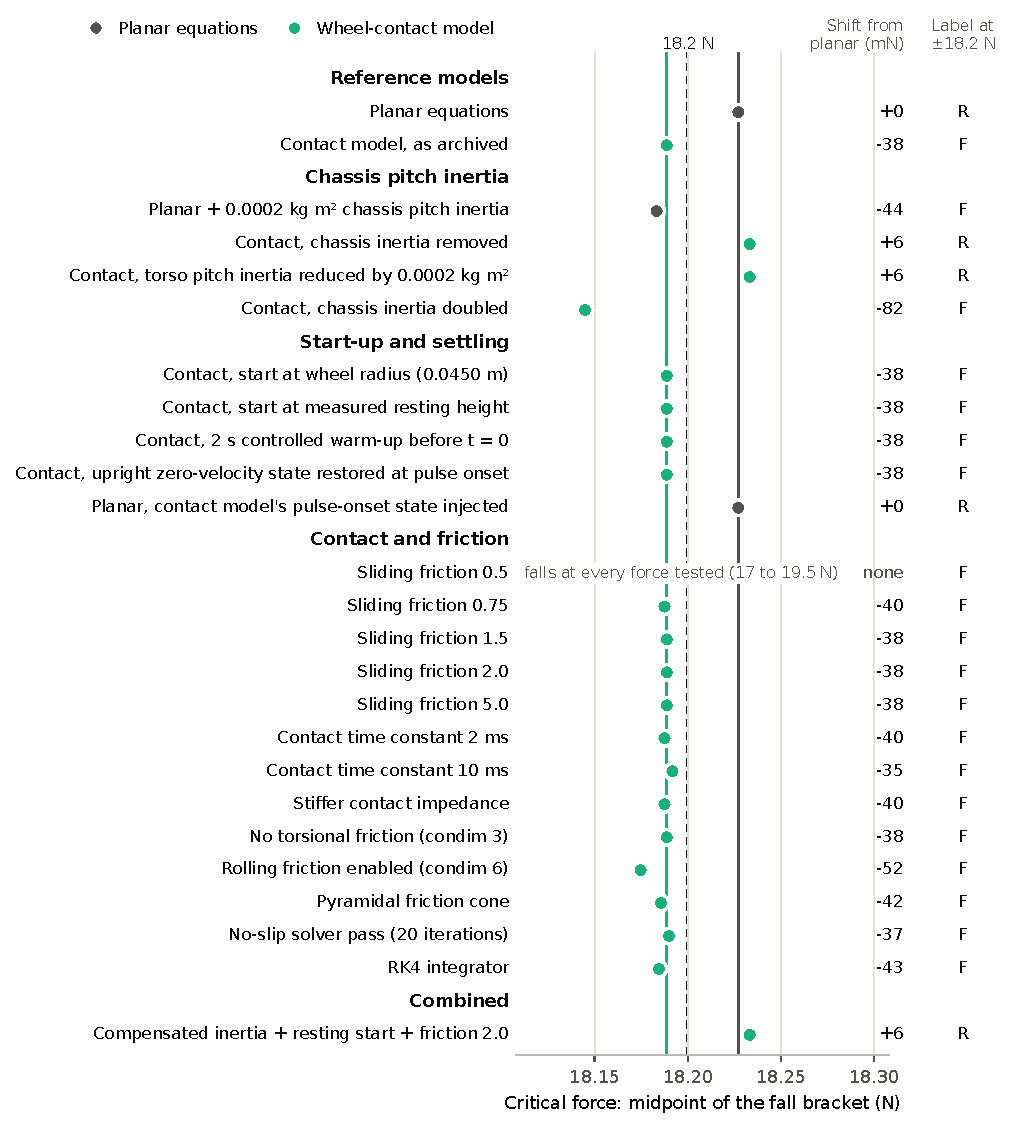
\includegraphics[width=\linewidth,height=.65\textheight,keepaspectratio]{../../figures/fu_fig01_boundary_shift.pdf}
\caption{Critical push force for each of the 25 diagnostic models at a 0.5 N m torque limit, zero initial tilt and a 0.125 ms physics step: the two unmodified references, 22 variants that each change one declared assumption, and one combined variant that changes three. Each dot is the midpoint of a bisection bracket 0.61 mN wide; solid vertical lines mark the unmodified planar (dark grey) and wheel-contact (green) models, and the dashed line marks the disputed 18.2 N cell. The numeric columns give the shift from the planar bracket in millinewtons and the label at +18.2 and -18.2 N at the 0.0625 ms confirmation step (R recovered, F fallen). Nothing is fitted, and no variant replaces the archived model.}
\end{figure}
\textbf{Table S2. Fall brackets at 0.125 ms and labels at \ensuremath{\pm}18.2 N at 0.0625 ms (R recovered, F fallen)}
\begin{longtable}{p{0.423\linewidth}p{0.225\linewidth}p{0.153\linewidth}p{0.099\linewidth}}
\toprule
Variant & Bracket (N) & Shift from planar (mN) & Label \\ \midrule \endhead
Planar equations & 18.2268 to 18.2274 & +0.0 & R \\
Contact model, as archived & 18.1884 to 18.1890 & -38.5 & F \\
Planar + 0.0002 kg m\textsuperscript{2} chassis pitch inertia & 18.1829 to 18.1835 & -43.9 & F \\
Contact, chassis inertia removed & 18.2329 to 18.2335 & +6.1 & R \\
Contact, torso pitch inertia reduced by 0.0002 kg m\textsuperscript{2} & 18.2329 to 18.2335 & +6.1 & R \\
Contact, chassis inertia doubled & 18.1444 to 18.1450 & -82.4 & F \\
Contact, start at wheel radius (0.0450 m) & 18.1884 to 18.1890 & -38.5 & F \\
Contact, start at measured resting height & 18.1884 to 18.1890 & -38.5 & F \\
Contact, 2 s controlled warm-up before t = 0 & 18.1884 to 18.1890 & -38.5 & F \\
Contact, upright zero-velocity state restored at pulse onset & 18.1884 to 18.1890 & -38.5 & F \\
Planar, contact model's pulse-onset state injected & 18.2268 to 18.2274 & +0.0 & R \\
Sliding friction 0.5 & Falls at 17.0, \ensuremath{\pm}18.2, 19.5 & none & F \\
Sliding friction 0.75 & 18.1871 to 18.1877 & -39.7 & F \\
Sliding friction 1.5 & 18.1884 to 18.1890 & -38.5 & F \\
Sliding friction 2.0 & 18.1884 to 18.1890 & -38.5 & F \\
Sliding friction 5.0 & 18.1884 to 18.1890 & -38.5 & F \\
Contact time constant 2 ms & 18.1871 to 18.1877 & -39.7 & F \\
Contact time constant 10 ms & 18.1914 to 18.1920 & -35.4 & F \\
Stiffer contact impedance & 18.1871 to 18.1877 & -39.7 & F \\
No torsional friction (condim 3) & 18.1884 to 18.1890 & -38.5 & F \\
Rolling friction enabled (condim 6) & 18.1743 to 18.1749 & -52.5 & F \\
Pyramidal friction cone & 18.1853 to 18.1859 & -41.5 & F \\
No-slip solver pass (20 iterations) & 18.1896 to 18.1902 & -37.2 & F \\
RK4 integrator & 18.1841 to 18.1847 & -42.7 & F \\
Compensated inertia + resting start + friction 2.0 & 18.2329 to 18.2335 & +6.1 & R \\
\bottomrule
\end{longtable}
A bracket gives the largest tested force without a fall and the smallest with one. It is a property of this model, controller, torque limit and pulse; it is not a disturbance rating. Shifts smaller than the bracket width cannot be distinguished from zero.

\clearpage
\section*{3 Inertia: the label follows the chassis, not the simulator}
\begin{figure}[htbp]
\centering
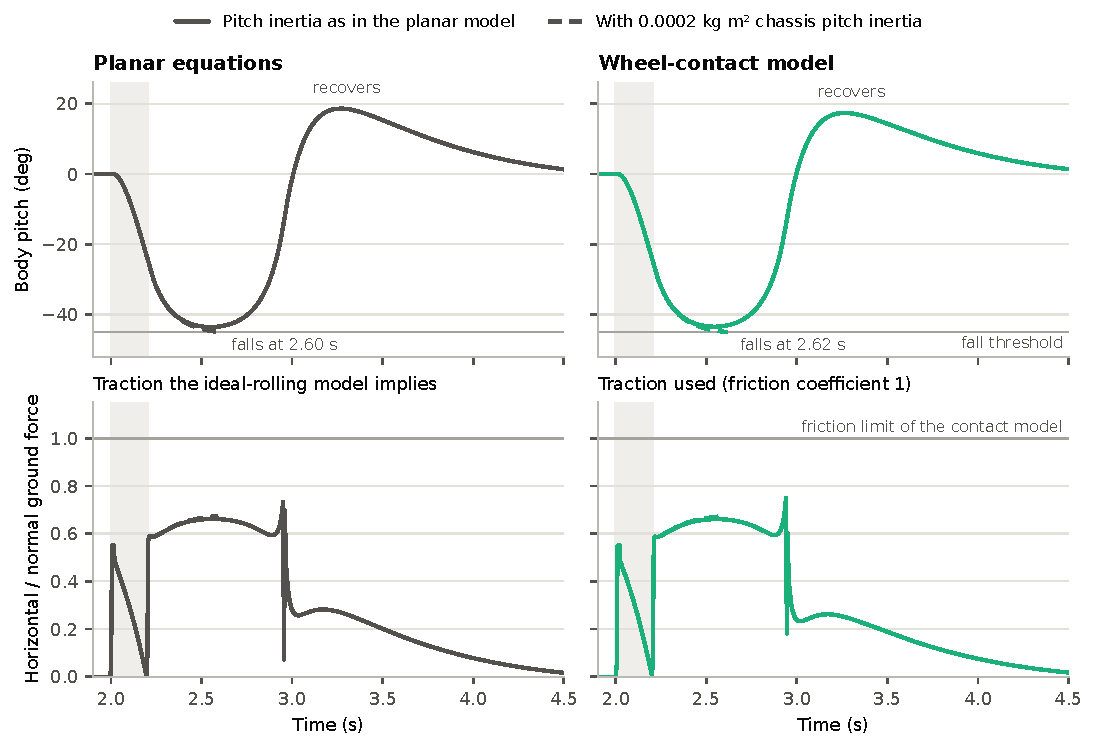
\includegraphics[width=\linewidth,height=.65\textheight,keepaspectratio]{../../figures/fu_fig02_boundary_mechanism.pdf}
\caption{The disputed +18.2 N cell at the 0.0625 ms confirmation step; the push acts in the shaded interval. Left: planar equations (dark grey); right: wheel-contact model (green), the plant colours of the critical-force figure. Top: body pitch. In both simulators the run recovers with the planar pitch inertia (solid) and falls when 0.0002 kg m\textsuperscript{2} of chassis pitch inertia is present (dashed): the label follows the inertia, not the simulator. The archived contact model is the dashed green curve. Bottom: ratio of horizontal to normal ground force. On the left it is the traction the ideal-rolling equations imply but never limit; on the right it is the traction the contact model uses. All four curves stay below the contact model's friction limit of 1 (largest value 0.75), so the wheels do not slide. The push tips the body backwards; a fall is declared at -45 deg. Curves end at a fall and are sampled every 5 ms.}
\end{figure}
The planar equations give the pitching assembly an inertia about the axle of I + m l\textsuperscript{2} = 0.05088 kg m\textsuperscript{2}. The contact model splits the 0.35 kg base into two wheels and a 0.11 kg chassis that is rigidly joined to the body and has its own inertia of 0.0002 kg m\textsuperscript{2} about each axis. Its mass sits on the axle and is already counted in the base mass; its pitch inertia is additional, an increase of 0.39\%.

Four variants isolate this term. Removing the chassis inertia from the contact model moves its bracket from -38.5 to +6.1 mN relative to the planar model, and the contact model then recovers at +18.2 and -18.2 N. Subtracting 0.0002 kg m\textsuperscript{2} from the body pitch inertia instead gives the identical bracket. Adding 0.0002 kg m\textsuperscript{2} to the planar body inertia moves the planar bracket by -43.9 mN, and the planar model then falls in both cells. Doubling the chassis inertia moves the contact bracket to -82.4 mN.

The response is linear over this range: -223, -220 and -220 N per kg m\textsuperscript{2} from three non-overlapping increments of 0.0002 kg m\textsuperscript{2} (removing it from the contact model, adding a second one to the contact model, adding one to the planar model), a mean of -221 N per kg m\textsuperscript{2}, or about -44 mN for the chassis term. Both simulators therefore agree on how the boundary depends on pitch inertia. With the inertia matched, the contact bracket lies +6.1 mN from the planar one (0.033\%), on the other side; that residual is the combined effect of everything else in the contact model. The inertia effect is therefore slightly larger than the gap it explains.

The direction is physically plausible but is reported as an observation. The fixed LQR gain was designed for the planar inertia, and under a saturated torque a body with more pitch inertia is both tipped and righted more slowly. In this cell the net effect is a smaller recoverable push. No claim is made that more inertia lowers the boundary in general.

\clearpage
\section*{4 Start-up and settling}
The contact model starts with the axle at 0.0452 m and comes to rest at 0.04499 m, a drop of 0.21 mm; first contact is recorded at 10 ms. In the force slices the robot starts exactly upright, so this drop is symmetric: it excites vertical motion only. At the start of the pulse, 2 s later, the sampled position, speed, pitch and pitch rate are all exactly zero and no slip has been recorded.

Four contact variants test settling directly: starting at the wheel radius, starting at the measured resting height, running a 2 s controlled warm-up before time zero, and restoring an exactly upright zero-velocity state at the instant the pulse begins. All four give the same bracket and the same fall time at 18.2 N as the unmodified contact model. Injecting the contact model's pulse-onset state into the planar model also changes nothing, because that state is zero. Settling is therefore ruled out for these two cells. The test does not cover starts with an initial tilt, where a drop is not symmetric; the archived start-up slice showed no disagreement there.

\clearpage
\section*{5 Contact, friction and the traction the planar model assumes}
13 variants change the contact model. Raising sliding friction to 1.5, 2 or 5, or removing torsional friction, leaves the bracket unchanged to the last bisection step. The other settings (friction 0.75, a 2 ms or 10 ms contact time constant, a stiffer impedance, a pyramidal friction cone, a no-slip solver pass, the RK4 integrator and rolling friction) move it by between -14.0 mN (rolling friction enabled (condim 6)) and +3.1 mN (contact time constant 10 ms) relative to the unmodified contact model. None changes the label at 18.2 N. The largest of these shifts is about a third of the 44.6 mN inertia effect and the rest are under a tenth of it; that is the size of contact-model sensitivity at this boundary.

Friction matters only when it is too low. The planar equations assume ideal rolling and never limit traction, but the ground force they imply can be computed from the trajectory. Its ratio to the normal force peaks at 0.59 for a 17 N push, 0.64 at 18 N and 0.73 at 18.2 N, where the long recovery near the boundary unloads the wheels to 6.5 N. The contact model with friction 1 uses at most 0.55 of its limit during the pulse and its sampled slip stays below 0.6 mm/s. With friction 0.75 the bracket moves by -1.2 mN. With friction 0.5, below the implied demand, the wheels slide at about 0.2 m/s and the robot falls at all three forces tested (17.0, \ensuremath{\pm}18.2 and 19.5 N), so no transition lies in the bracket.

This gives the planar model a stated domain of validity that it did not have before: near this boundary it describes a robot on a surface whose friction coefficient is at least about 0.75. That is a requirement to check on hardware, not a property the simulations establish.

\clearpage
\section*{6 What the diagnosis does and does not show}
The two disagreements are a modelling difference of known size, not a numerical artefact and not a contact effect. Two simulators that agree on how the boundary depends on inertia were given inertias that differ by 0.39\%, and the 18.2 N grid force lies in the 38.5 mN between their boundaries.

\textbf{Table S3. Post hoc consistency check at all three force boundaries (critical forces in N, shifts in mN relative to planar)}
\begin{longtable}{p{0.099\linewidth}p{0.117\linewidth}p{0.117\linewidth}p{0.126\linewidth}p{0.144\linewidth}p{0.153\linewidth}p{0.144\linewidth}}
\toprule
Limit (N m) & Planar & Contact & Contact shift & Inertia matched & Grid forces in gap & Archived labels \\ \midrule \endhead
0.3 & 11.8837 & 11.8581 & -25.6 & +3.4 & none & 22/22 \\
0.5 & 18.2271 & 18.1887 & -38.5 & +6.1 & 18.2 & 22/22 \\
0.7 & 21.8495 & 21.8145 & -35.0 & +3.4 & none & 22/22 \\
\bottomrule
\end{longtable}
If chassis inertia is the cause, it should act at every force boundary, and the archived zoom labels should follow from where the 0.05 N grid happens to fall. A post hoc check, designed after the main diagnostics, brackets the planar, contact, inertia-added and inertia-removed models at the 0.3 and 0.7 N m boundaries as well (168 further integrations). The contact boundary is lower than the planar one at all three limits, by 25.6, 38.5 and 35.0 mN. Matching the inertia reverses the sign at every limit, leaving the contact boundary +3.4, +6.1 and +3.4 mN from the planar one: a small, consistent residual from the rest of the contact model. The brackets reproduce the archived label of both models in all 66 zoom cells of the three slices: the only grid forces that lie between the two boundaries are the two disputed ones. The archived agreement at 0.3 and 0.7 N m is therefore a matter of grid placement, and the critical-force difference is the better summary of simulator agreement than a count of matching cells.

The diagnosis does not make either model correct. Whether a real chassis contributes 0.0002 kg m\textsuperscript{2} is a property of hardware that has not been built or measured. A shift of 0.2\% in critical force is far below any plausible uncertainty in an identified pitch inertia or an applied push, so for hardware purposes the two models make the same prediction at this boundary, provided traction is adequate. The archived contact model is left unchanged, with its chassis inertia, and no variant is adopted as a correction.

\clearpage
\section*{7 Noisy payload comparison: protocol and port verification}
The planar comparison of fixed and payload-aware LQR used nine reserved loads (0.35, 0.65 and 1.15 kg at 0.14, 0.26 and 0.36 m), two disturbance scenarios, three sensing profiles and 30 noise seeds: 1,620 paired trials per controller. Both scenarios pair a 7 degree initial tilt with an opposing 12 N push; they differ in torque limit, 0.6 N m in one and 0.3 N m in the other, with the signs mirrored. The profiles add Gaussian noise of 0.75 degrees to pitch and 3 deg/s to pitch rate and feed the controller the raw packet, a two-state Kalman estimate, or that estimate with a 10 ms packet delay. Both controllers use Q = diag(12,2,120,2) and R = 1; the payload-aware gain is designed for the true load.

The repeat changes one thing: the plant. The protocol, saved before any noisy contact run, copies the conditions, gains and seeds unchanged and declares in advance the paired analysis, a per-plant sign test, breakdowns by scenario, profile, mass and height, one example trajectory, and a persistence criterion: the reduction persists if payload-aware LQR has fewer falls than fixed LQR, and prevents more falls than it introduces, at both contact physics steps (0.25 and 0.5 ms). The criterion checks direction only, and the 0.5 ms run is a step-size check of the same deterministic model with the same seeds, not an independent replicate. The contact plant is the unmodified loaded model of the boundary and payload report, with friction 1, the archived chassis inertia and no warm-up. Measurements are the true position, speed, pitch and pitch rate of its base, with noise and delay applied by the same code path as for the planar plant.

The sensing pipeline exists in JavaScript. It was ported line for line to Python: the 32-bit linear congruential generator, the Box-Muller pairs, the packet queue and the scalar Kalman updates. Before any contact result was used, the port was run on the planar plant for every archived fixed and payload-aware record. All 3,240 outcomes match the archive; the largest differences are 6.2 \ensuremath{\times} 10⁻⁸ degrees in peak tilt and 1.2 \ensuremath{\times} 10⁻¹⁰ (N m)\textsuperscript{2} s in the squared-torque integral. The contact plant therefore receives the same noise sequence as the planar plant, trial by trial.

\clearpage
\section*{8 Falls and paired transitions}
\begin{figure}[htbp]
\centering
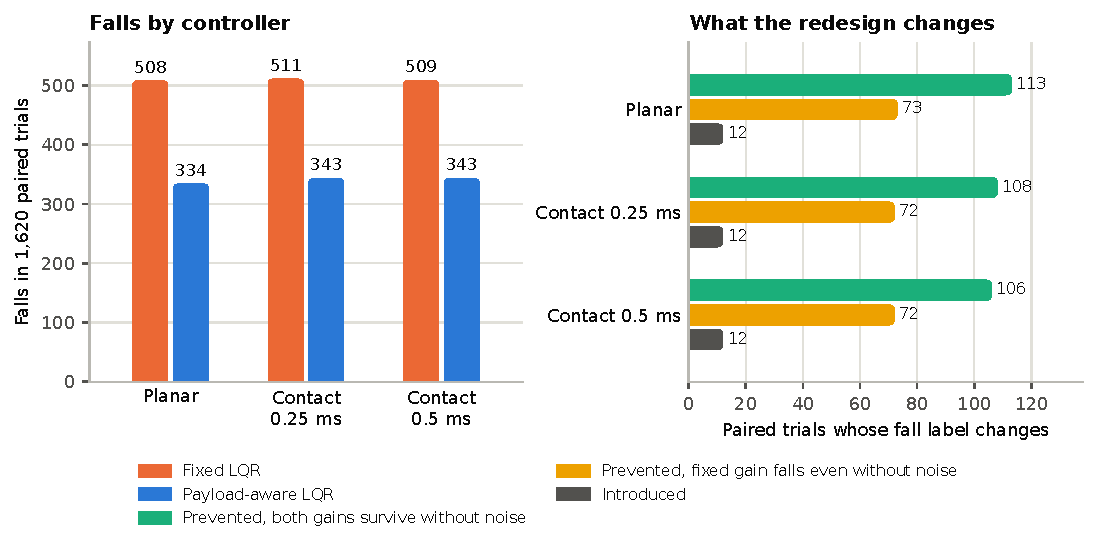
\includegraphics[width=\linewidth,height=.65\textheight,keepaspectratio]{../../figures/fu_fig03_noisy_falls.pdf}
\caption{Noisy fixed-versus-payload-aware comparison on the same 1,620 condition and seed pairs in each plant. Left: falls by controller. Right: paired trials whose fall label changes when the fixed gain is replaced by the exact-load gain. Prevented falls are split by what happens with exact state feedback at the same load and disturbance: both gains survive without noise, or the fixed gain falls even without noise. Every introduced fall is in conditions that both gains survive without noise. This split follows the fixed gain; the per-controller split is in the text. The planar counts equal the archived JavaScript results record for record. The contact runs use physics steps of 0.25 and 0.5 ms with 200 Hz control. Every fall in every plant occurs at the 0.3 N m torque limit. Counts describe this grid, not deployment probabilities.}
\end{figure}
\textbf{Table S4. Falls in 1,620 paired trials and paired transitions from fixed to payload-aware LQR}
\begin{longtable}{p{0.234\linewidth}p{0.135\linewidth}p{0.135\linewidth}p{0.126\linewidth}p{0.126\linewidth}p{0.144\linewidth}}
\toprule
Plant & Fixed falls & Aware falls & Prevented & Introduced & Net reduction \\ \midrule \endhead
Planar & 508 & 334 & 186 & 12 & 34\% \\
Contact, 0.25 ms & 511 & 343 & 180 & 12 & 33\% \\
Contact, 0.5 ms & 509 & 343 & 178 & 12 & 33\% \\
\bottomrule
\end{longtable}
The declared criterion is met at both contact steps. At 0.25 ms the redesign removes 168 of 511 falls (33\%); at 0.5 ms, 166 of 509 (33\%). The planar reduction was 174 of 508 (34\%). As in the planar model, the net figure hides regressions: the redesign introduces 12 falls at 0.25 ms and 12 at 0.5 ms.

Every fall, in every plant and under every profile, occurs in the 0.3 N m scenario. No trial in the 0.6 N m scenario falls, under either gain. The comparison therefore rests on one disturbance at one torque limit, and the 810 pairs (1,620 trials) at 0.6 N m contribute only to the survivor statistics. Section 10 shows why: at 0.6 N m both gains' exact-feedback boundaries are at least 19.6 N, far above the 12 N push. The declared exact two-sided sign test on the discordant pairs gives p = 1.3 \ensuremath{\times} 10⁻³⁹ at 0.25 ms, 4.4 \ensuremath{\times} 10⁻³⁹ at 0.5 ms and 2.9 \ensuremath{\times} 10⁻⁴¹ in the planar port.This summarises seed-level evidence inside one model. The 1,620 pairs share nine loads and two scenarios, so the test says nothing about a population of robots, loads or floors.

No noisy contact-model run meets the strict one-second recovery dwell, as in the planar model: persistent measurement noise keeps every survivor moving. Survivors are therefore labelled upright but unsettled, and the fall is the primary outcome.

\clearpage
\section*{9 Exact-feedback control at the same conditions}
\begin{figure}[htbp]
\centering
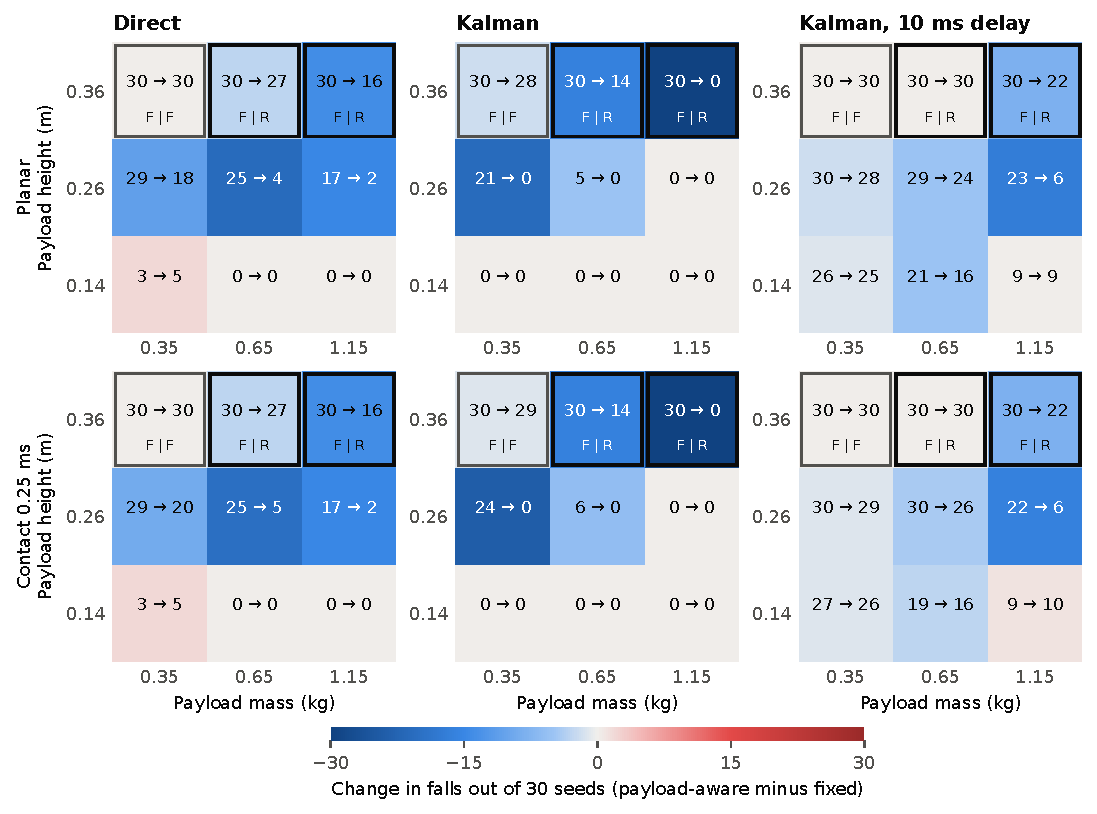
\includegraphics[width=\linewidth,height=.65\textheight,keepaspectratio]{../../figures/fu_fig04_noisy_map.pdf}
\caption{Where the redesign changes falls: the 0.3 N m scenario (initial tilt -7 deg, +12 N push), for all nine loads and three sensing profiles, in the planar model (top) and the contact model at 0.25 ms (bottom). Each cell prints fixed-gain falls → payload-aware falls out of 30 paired seeds; colour is their difference, blue where the redesign removes falls. With exact state feedback both gains recover at every unmarked load. At the two loads marked F | R (0.65 and 1.15 kg at 0.36 m, three squares each) the fixed gain falls even with exact feedback and the payload-aware gain does not; at the load marked F | F (0.35 kg at 0.36 m) both fall. The 0.6 N m scenario is not drawn: no trial fell there under any gain, profile or plant. The 0.5 ms contact step check is in results/mujoco\_followup/cells.csv.}
\end{figure}
The archived ideal-sensing comparisons found no fall label changed by the redesign, in 216 planar and 36 contact conditions. Those conditions used different initial tilts and forces from the two noisy scenarios, at the same two torque limits. To separate the effect of the redesign from the effect of noise, the two noisy scenarios were run at all nine loads with exact state feedback (zero noise, zero delay) in all three plants: 108 deterministic runs. This control was designed after the noisy results were known. Its planar runs reproduce the archived JavaScript trial function in all 36 records.

\textbf{Table S5. Exact-feedback outcome of the 18 load and scenario conditions, identical in all three plants}
\begin{longtable}{p{0.243\linewidth}p{0.108\linewidth}p{0.549\linewidth}}
\toprule
With exact feedback & Conditions & Which \\ \midrule \endhead
Both gains recover & 15 & all nine loads at 0.6 N m; 0.3 N m: 0.35 kg at 0.14 m, 0.35 kg at 0.26 m, 0.65 kg at 0.14 m, 0.65 kg at 0.26 m, 1.15 kg at 0.14 m, 1.15 kg at 0.26 m \\
Only the fixed gain falls & 2 & 0.3 N m: 0.65 kg at 0.36 m, 1.15 kg at 0.36 m \\
Both gains fall & 1 & 0.3 N m: 0.35 kg at 0.36 m \\
\bottomrule
\end{longtable}
With exact feedback the redesign changes the fall label in two of the 18 conditions, both at 0.3 N m and 0.36 m: at 0.65 and 1.15 kg the fixed gain falls and the payload-aware gain recovers. It changes nothing in the other 16. The classification is the same in the planar model and at both contact steps. Taken with the earlier grids, the redesign changes the fall label with exact feedback in 2 of 234 distinct planar conditions and 2 of 54 contact-model conditions, always by preventing a fall.

\textbf{Table S6. Noisy pairs split by the exact-feedback outcome of the same load and disturbance: falls (fixed → payload-aware) and falls prevented}
\begin{longtable}{p{0.162\linewidth}p{0.18\linewidth}p{0.108\linewidth}p{0.108\linewidth}p{0.216\linewidth}p{0.126\linewidth}}
\toprule
Plant & Both gains survive without noise & Prevented & Introduced & Fixed gain falls without noise & Prevented \\ \midrule \endhead
Planar & 238 → 137 & 113 & 12 & 270 → 197 & 73 \\
Contact, 0.25 ms & 241 → 145 & 108 & 12 & 270 → 198 & 72 \\
Contact, 0.5 ms & 239 → 145 & 106 & 12 & 270 → 198 & 72 \\
\bottomrule
\end{longtable}
Table S6 sorts every pair by what both gains do without noise. In the 15 conditions that both gains survive without noise, the redesign reduces falls from 241 to 145 in the contact model at 0.25 ms (planar 238 to 137), preventing 108 and introducing 12; all of these falls lie in the six 0.3 N m conditions at 0.14 and 0.26 m, and every introduced fall is in this group. The other 72 prevented falls (planar 73) are in the three conditions where the fixed gain falls without noise. Of these, the two conditions where the payload-aware gain recovers without noise contribute 71 in every plant, and there noise makes the payload-aware gain fall in 109 of 180 trials (planar 109).

\textbf{Table S7. Noisy falls per controller, split by whether the same controller falls at the same load and disturbance without noise}
\begin{longtable}{p{0.18\linewidth}p{0.18\linewidth}p{0.18\linewidth}p{0.18\linewidth}p{0.18\linewidth}}
\toprule
Plant & Fixed: survives without noise & Aware: survives without noise & Fixed: falls without noise & Aware: falls without noise \\ \midrule \endhead
Planar & 238 & 246 & 270 & 88 \\
Contact, 0.25 ms & 241 & 254 & 270 & 89 \\
Contact, 0.5 ms & 239 & 254 & 270 & 89 \\
\bottomrule
\end{longtable}
This split is not symmetric, because it classifies the payload-aware gain's falls by what the fixed gain does. Table S7 classifies each controller by its own exact-feedback outcome. Counted that way, the redesign does not reduce the falls that noise causes: in the contact model 241 fixed-gain and 254 payload-aware falls occur in conditions that the same controller survives without noise. The whole net reduction comes from the conditions in which the fixed gain falls without noise and the payload-aware gain mostly does not. Neither split, on its own, says why; the boundary measurement of Section 10 does.

\clearpage
\section*{10 The exact-feedback boundary of both gains}
\begin{figure}[htbp]
\centering
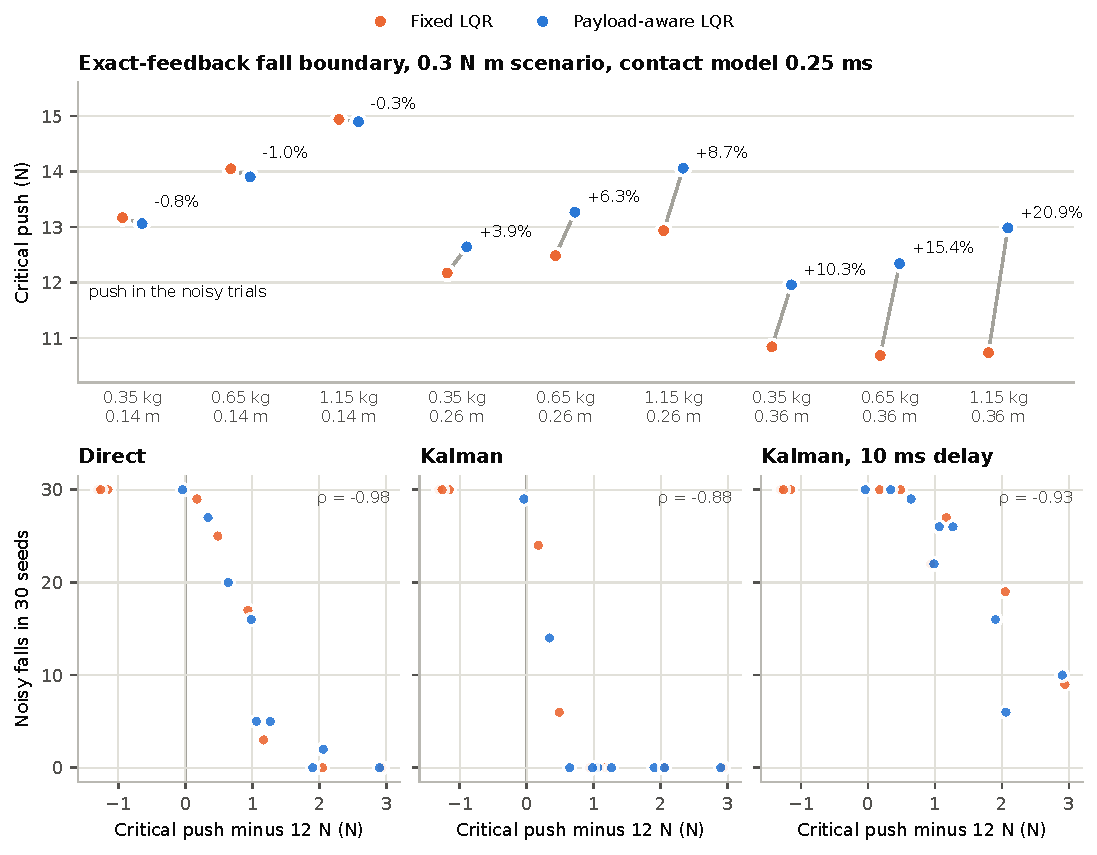
\includegraphics[width=\linewidth,height=.65\textheight,keepaspectratio]{../../figures/fu_fig08_exact_boundary.pdf}
\caption{What the redesign changes without noise, and how that predicts the noisy falls. Top: the smallest push that makes each gain fall with exact state feedback, at the -7 deg tilt and 0.3 N m limit of the noisy scenario, found by bisection to 9.8 mN in the contact model at 0.25 ms (the planar model and the 0.5 ms step differ by at most 0.04 N). Labels give the payload-aware boundary relative to the fixed one. The dashed line is the 12 N push of the noisy trials: where both dots lie above it, both gains recover without noise. Bottom: noisy falls of each gain against the distance from 12 N to that gain's own boundary, one dot per load and gain, by sensing profile. Both gains follow one relationship; ρ is the Spearman rank correlation over all 18 dots. Post hoc analysis.}
\end{figure}
A fall label at one push says only on which side of the boundary that push lies. This post hoc analysis, added after an internal review of the integrated manuscript, measures the boundary itself. For each load, both noisy scenarios, both gains and all three plants, bisection over the push magnitude between 0 and 40 N finds, to 9.8 mN, the smallest push that makes the robot fall with exact state feedback; tilt, torque limit, pulse, gains and fall rule are those of the noisy study (2,988 integrations). Planar runs also scan 0 to 40 N in 1 N steps and show a single fall transition, and every boundary is consistent with the archived exact-feedback label at 12 N.

\textbf{Table S8. Exact-feedback critical push (N) in the contact model at 0.25 ms; the noisy trials push with 12 N}
\begin{longtable}{p{0.171\linewidth}p{0.122\linewidth}p{0.122\linewidth}p{0.099\linewidth}p{0.122\linewidth}p{0.122\linewidth}p{0.099\linewidth}}
\toprule
Load & Fixed, 0.3 N m & Aware, 0.3 N m & Shift & Fixed, 0.6 N m & Aware, 0.6 N m & Shift \\ \midrule \endhead
0.35 kg, 0.14 m & 13.17 & 13.06 & -0.8\% & 23.69 & 23.49 & -0.8\% \\
0.35 kg, 0.26 m & 12.17 & 12.64 & +3.9\% & 21.84 & 22.70 & +3.9\% \\
0.35 kg, 0.36 m & 10.84 & 11.96 & +10.3\% & 19.60 & 21.61 & +10.2\% \\
0.65 kg, 0.14 m & 14.05 & 13.90 & -1.0\% & 25.59 & 25.37 & -0.9\% \\
0.65 kg, 0.26 m & 12.49 & 13.27 & +6.3\% & 22.75 & 24.16 & +6.2\% \\
0.65 kg, 0.36 m & 10.69 & 12.34 & +15.4\% & 19.64 & 22.68 & +15.5\% \\
1.15 kg, 0.14 m & 14.94 & 14.90 & -0.3\% & 27.87 & 27.72 & -0.5\% \\
1.15 kg, 0.26 m & 12.93 & 14.06 & +8.7\% & 24.02 & 26.12 & +8.7\% \\
1.15 kg, 0.36 m & 10.74 & 12.98 & +20.9\% & 20.11 & 24.34 & +21.0\% \\
\bottomrule
\end{longtable}
The redesign moves the boundary by an amount that grows with mounting height and mass (Table S8, Figure 5). It raises it by 3.9\% to 8.7\% at 0.26 m and by 10.2\% to 21.0\% at 0.36 m, and lowers it by 0.3\% to 1.0\% at 0.14 m, at both torque limits. The planar model and both contact steps give the same boundaries to within 0.04 N. At the two upper heights these shifts are twenty to a hundred times the 0.2\% that separates the two simulators at the boundary of Section 2, yet almost none of them changes a label on a fixed grid, because a label changes only when a test force happens to lie between the two boundaries. That happens at 0.65 and 1.15 kg at 0.36 m and 12 N, and nowhere on the 216-condition ideal grid.

The boundaries also account for the noisy results. At 0.6 N m both gains' boundaries are at least 19.6 N, and no noisy trial falls. At 0.3 N m the 12 N push lies 0.17 to 0.93 N below the fixed gain's boundary at 0.26 m and further below the payload-aware one. Plotted against the distance from 12 N to its own boundary, each gain's noisy fall count falls on one decreasing relationship for both gains (Figure 5, bottom; Spearman rank correlation -0.98 to -0.88 over the 18 load and gain points, per plant and profile). For example, in the contact model with direct measurements the fixed gain at 1.15 kg and 0.26 m and the payload-aware gain at 1.15 kg and 0.36 m have nearly the same margin and nearly the same number of falls. The noisy fall reduction is therefore what a boundary shift looks like when noise spreads the effective disturbance around a push close to the boundary. This reading is post hoc and rests on 18 points per profile; it predicts that the noisy benefit would vanish for pushes far below both boundaries and turn into a deterministic difference for pushes between them.

\clearpage
\section*{11 A noisy fall that the redesign prevents}
\begin{figure}[htbp]
\centering
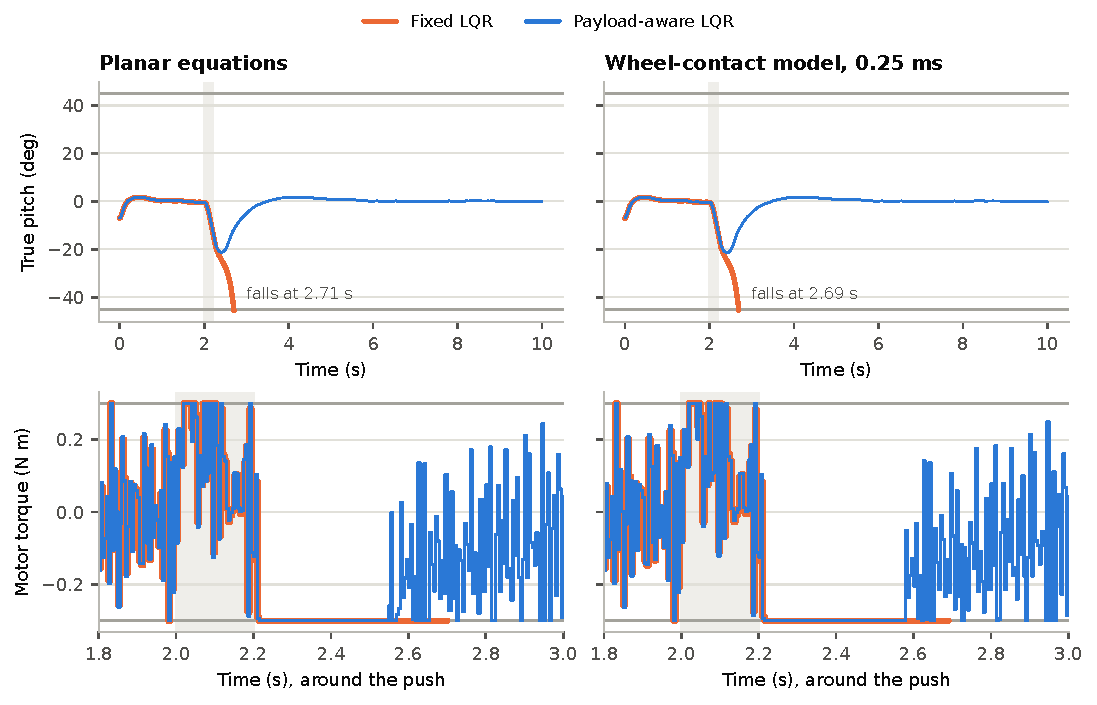
\includegraphics[width=\linewidth,height=.65\textheight,keepaspectratio]{../../figures/fu_fig06_noise_induced_fall.pdf}
\caption{A noisy fall that the redesign prevents. The selection rule was written after the noisy results were known and deliberately picks a favourable case: the condition that both gains survive without noise and in which the redesign prevents the most falls in the contact model (0.35 kg at 0.26 m, 0.3 N m scenario, kalman profile; 24 of 30 seeds prevented), and the lowest seed at which the fixed gain falls and the payload-aware gain survives in both plants (seed index 0). Top: true pitch over the whole run. Bottom: the torque command, held over each 5 ms interval, from 1.8 to 3.0 s; the fixed-gain trace is drawn wider underneath so both stay visible where they coincide at the limit. Grey lines mark the \ensuremath{\pm}45 deg fall threshold and the \ensuremath{\pm}0.3 N m torque limit. Both plants receive the same noise sequence. The payload-aware runs stay upright but, like every noisy survivor, do not meet the recovery dwell.}
\end{figure}
Figure 6 shows one noisy fall that the redesign prevents. The selection rule was written after the noisy results were known and picks a favourable case: the condition that both gains survive without noise and in which the redesign prevents the most falls in the contact model (0.35 kg at 0.26 m, 0.3 N m, kalman profile; 24 of 30 seeds in the contact model and 21 in the planar model), and within it the lowest seed at which the fixed gain falls and the payload-aware gain survives in both plants (seed index 0). The fixed gain falls at 2.71 s in the planar model and 2.69 s in the contact model; the payload-aware gain stays upright in both. Without noise, both gains recover in this cell.

The same ordering by mounting height appears in the noisy counts. In the conditions both gains survive without noise, the redesign prevents 13 falls in the contact model at 0.14 m and introduces 12, little net effect where its boundary barely moves (planar 15 and 11). At 0.26 m it prevents 95 and introduces 0 (planar 98 and 1). The single exact-feedback runs at 12 N agree: at 0.14 m the two gains reach the same peak tilt within 0.15 degrees and spend the same time at the torque limit to within one control interval; at 0.26 m the fixed gain recovers with 0.8 to 2.1 degrees more peak tilt. At 0.36 m the fixed gain falls at all three masses even without noise, and the payload-aware gain at one (0.35 kg).

Noise consumes much of the torque budget. With exact feedback, a surviving run at 0.3 N m spends a median of 0.04 s at the torque limit. Under noise, surviving contact-model runs at 0.3 N m spend a median 39\% of the run at the limit with direct measurements, 11\% with the Kalman estimate and 70\% with the delayed estimate, where the command settles into a full-torque limit cycle (Figure 7 shows the same at 0.6 N m). Among the 287 contact-model pairs in the six noise-affected cells in which both gains stay upright, the paired difference (payload-aware minus fixed) in time at the limit has a median of -0.09 (interquartile range -0.16 to +0.04) s, and in the squared-torque integral -0.0068 (interquartile range -0.0131 to +0.0127) (N m)\textsuperscript{2} s; the planar values are -0.09 (interquartile range -0.16 to +0.04) s and -0.0069 (interquartile range -0.0131 to +0.0120).

Survivor comparisons are conditional on both gains staying upright and describe nine loads, two disturbances and one noise level. They are consistent with the boundary reading of Section 10 but do not test it.

\clearpage
\section*{12 Protocol-selected example}
\begin{figure}[htbp]
\centering
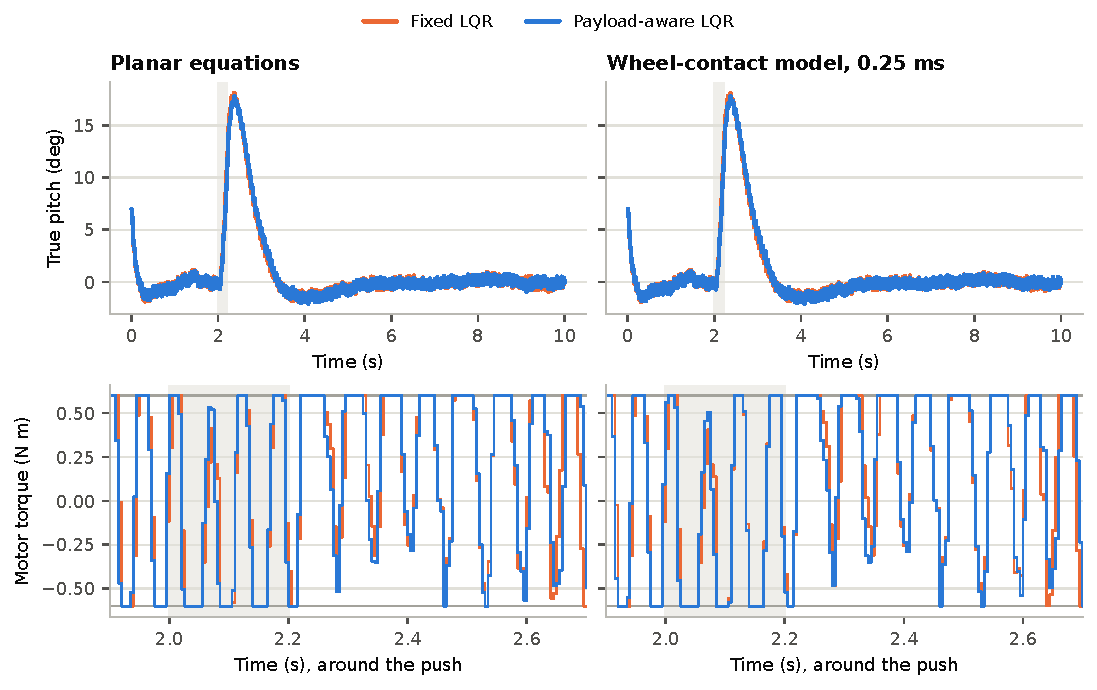
\includegraphics[width=\linewidth,height=.65\textheight,keepaspectratio]{../../figures/fu_fig05_noisy_example.pdf}
\caption{Protocol-selected noisy example, fixed before the runs: 0.65 kg at 0.26 m, 0.6 N m scenario (initial tilt +7 deg, -12 N push in the shaded interval), Kalman estimate with 10 ms packet delay, first seed. Top: true pitch over the whole run. Bottom: the torque command, held over each 5 ms interval, from 1.9 to 2.7 s; with this noise and delay it switches between the \ensuremath{\pm}0.6 N m limits (grey lines) for much of the run, so a full-length trace is unreadable. Both controllers and both plants receive the same noise sequence, and all four runs stay upright, as does every trial at 0.6 N m.}
\end{figure}
The protocol fixed one example before any noisy contact run (Figure 7): 0.65 kg at 0.26 m, the 0.6 N m scenario, the Kalman profile with a 10 ms delay and the first seed. Like every trial at 0.6 N m, all four runs stay upright. The example shows that the two plants respond almost identically to the same noise sequence, and that the redesign changes the response without changing the outcome.

Across all 1,097 pairs in which both controllers survive in the contact model at 0.25 ms, most of them at 0.6 N m, the payload-aware design changes median peak tilt by -0.49 (interquartile range -0.99 to -0.11) degrees, the squared-torque integral by +0.0261 (interquartile range -0.0253 to +0.0927) (N m)\textsuperscript{2} s and final-second tilt RMS by -0.001 (interquartile range -0.004 to +0.003) degrees. In the planar port the 1,100 mutual survivors give -0.49 (interquartile range -1.00 to -0.11) degrees, +0.0261 (interquartile range -0.0220 to +0.0930) (N m)\textsuperscript{2} s and 0.000 (interquartile range -0.004 to +0.003) degrees. These are conditional on mutual survival and exclude every fall; they complement the fall counts and cannot replace them.

\clearpage
\section*{13 Agreement between plants, step sensitivity and repeatability}
\begin{figure}[htbp]
\centering
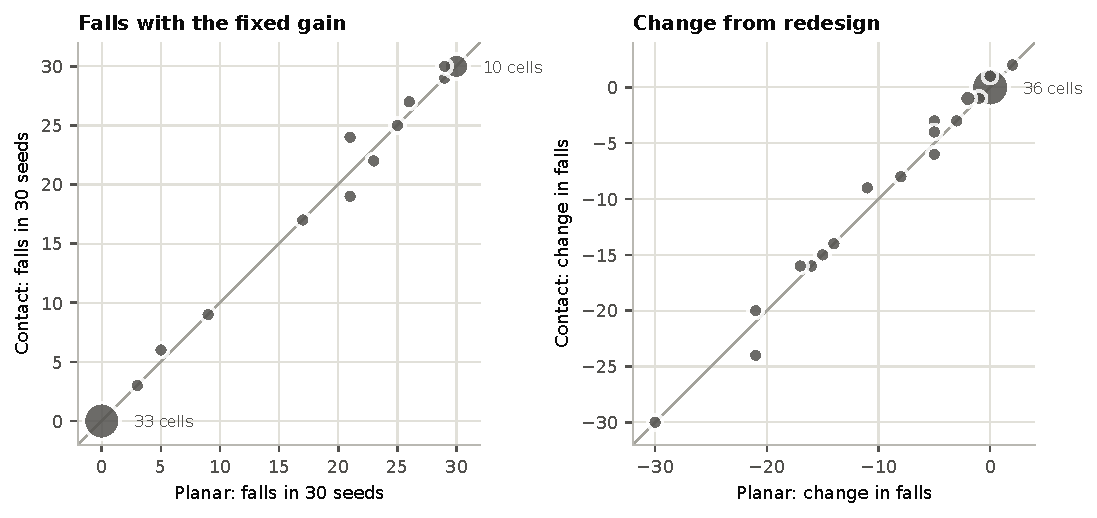
\includegraphics[width=\linewidth,height=.65\textheight,keepaspectratio]{../../figures/fu_fig07_plant_agreement.pdf}
\caption{Agreement between plants, cell by cell. Each of the 54 cells is one load, scenario and sensing profile with 30 seeds; dot area grows with the number of coincident cells, and the 27 cells of the 0.6 N m scenario all sit at the origin. Left: falls under the fixed gain in the planar model against the contact model (0.25 ms). Right: net change in falls when the payload-aware gain replaces the fixed gain (payload-aware minus fixed); negative values are net reductions, prevented minus introduced. Points on the diagonal agree exactly. The direction of the change (fewer, equal or more falls) is the same in 53 of 54 cells.}
\end{figure}
The two plants agree on where falls occur and where the redesign helps (Figure 8). Here a cell is one load, scenario and sensing profile with 30 seeds. The direction of the change in falls (fewer, equal or more) is the same in the planar model and the contact model at 0.25 ms in 53 of 54 cells. A noisy closed loop near a fall boundary amplifies small numerical differences, so an individual seed can fall in one plant or at one step and survive in another. Individual fall labels agree between the planar port and the contact model at 0.25 ms in 3,218 of 3,240 trials, between the two contact steps in 3,236, and between the planar port and the contact model at 0.5 ms in 3,218. Aggregate and paired counts are the unit of comparison; they differ between the two contact steps by 2 fixed-gain falls and 0 payload-aware falls.

The contact runs were checkpointed by condition group and computed by parallel worker processes. To confirm that this cannot have changed a result, 12 groups (360 trials, every 18th group in sorted order) were recomputed from scratch in fresh processes; all 360 records are identical to the stored ones in all 24 fields. The two contact runs are complete repeats of the same model at two physics steps, not a selective audit, and do not amount to a convergence proof. The planar port uses one RK4 step per 5 ms control interval, as archived.

\textbf{Table S9. Falls by scenario (810 pairs each) and, since every fall is at 0.3 N m, by sensing profile (540 pairs each, both scenarios): fixed to payload-aware}
\begin{longtable}{p{0.333\linewidth}p{0.189\linewidth}p{0.189\linewidth}p{0.189\linewidth}}
\toprule
Group & Planar & Contact 0.25 ms & Contact 0.5 ms \\ \midrule \endhead
+7 deg, -12 N, 0.6 N m, all profiles & 0 to 0 & 0 to 0 & 0 to 0 \\
-7 deg, +12 N, 0.3 N m, all profiles & 508 to 334 & 511 to 343 & 509 to 343 \\
0.3 N m, Direct & 164 to 102 & 164 to 105 & 164 to 104 \\
0.3 N m, Kalman & 116 to 42 & 120 to 43 & 119 to 43 \\
0.3 N m, Kalman, 10 ms delay & 228 to 190 & 227 to 195 & 226 to 196 \\
\bottomrule
\end{longtable}
\clearpage
\section*{14 Complete per-cell table}
Table S10 gives every cell: one load, torque limit and sensing profile with 30 paired seeds. The exact-feedback column gives the outcome of the same load and disturbance without noise: R | R both gains recover, F | R only the fixed gain falls, F | F both fall, as in Figure 4. The same table, with prevented and introduced counts, is in results/mujoco\_followup/cells.csv.

\textbf{Table S10. Falls in 30 seeds, fixed to payload-aware, for every load, torque limit (N m) and sensing profile}
\begin{longtable}{p{0.171\linewidth}p{0.072\linewidth}p{0.198\linewidth}p{0.072\linewidth}p{0.126\linewidth}p{0.131\linewidth}p{0.131\linewidth}}
\toprule
Load & Limit & Profile & Exact & Planar & Contact 0.25 & Contact 0.5 \\ \midrule \endhead
0.35 kg, 0.14 m & 0.6 & Direct & R | R & 0 to 0 & 0 to 0 & 0 to 0 \\
0.35 kg, 0.14 m & 0.6 & Kalman & R | R & 0 to 0 & 0 to 0 & 0 to 0 \\
0.35 kg, 0.14 m & 0.6 & Kalman, 10 ms delay & R | R & 0 to 0 & 0 to 0 & 0 to 0 \\
0.35 kg, 0.14 m & 0.3 & Direct & R | R & 3 to 5 & 3 to 5 & 3 to 5 \\
0.35 kg, 0.14 m & 0.3 & Kalman & R | R & 0 to 0 & 0 to 0 & 0 to 0 \\
0.35 kg, 0.14 m & 0.3 & Kalman, 10 ms delay & R | R & 26 to 25 & 27 to 26 & 27 to 26 \\
0.35 kg, 0.26 m & 0.6 & Direct & R | R & 0 to 0 & 0 to 0 & 0 to 0 \\
0.35 kg, 0.26 m & 0.6 & Kalman & R | R & 0 to 0 & 0 to 0 & 0 to 0 \\
0.35 kg, 0.26 m & 0.6 & Kalman, 10 ms delay & R | R & 0 to 0 & 0 to 0 & 0 to 0 \\
0.35 kg, 0.26 m & 0.3 & Direct & R | R & 29 to 18 & 29 to 20 & 29 to 19 \\
0.35 kg, 0.26 m & 0.3 & Kalman & R | R & 21 to 0 & 24 to 0 & 23 to 0 \\
0.35 kg, 0.26 m & 0.3 & Kalman, 10 ms delay & R | R & 30 to 28 & 30 to 29 & 30 to 29 \\
0.35 kg, 0.36 m & 0.6 & Direct & R | R & 0 to 0 & 0 to 0 & 0 to 0 \\
0.35 kg, 0.36 m & 0.6 & Kalman & R | R & 0 to 0 & 0 to 0 & 0 to 0 \\
0.35 kg, 0.36 m & 0.6 & Kalman, 10 ms delay & R | R & 0 to 0 & 0 to 0 & 0 to 0 \\
0.35 kg, 0.36 m & 0.3 & Direct & F | F & 30 to 30 & 30 to 30 & 30 to 30 \\
0.35 kg, 0.36 m & 0.3 & Kalman & F | F & 30 to 28 & 30 to 29 & 30 to 29 \\
0.35 kg, 0.36 m & 0.3 & Kalman, 10 ms delay & F | F & 30 to 30 & 30 to 30 & 30 to 30 \\
0.65 kg, 0.14 m & 0.6 & Direct & R | R & 0 to 0 & 0 to 0 & 0 to 0 \\
0.65 kg, 0.14 m & 0.6 & Kalman & R | R & 0 to 0 & 0 to 0 & 0 to 0 \\
0.65 kg, 0.14 m & 0.6 & Kalman, 10 ms delay & R | R & 0 to 0 & 0 to 0 & 0 to 0 \\
0.65 kg, 0.14 m & 0.3 & Direct & R | R & 0 to 0 & 0 to 0 & 0 to 0 \\
0.65 kg, 0.14 m & 0.3 & Kalman & R | R & 0 to 0 & 0 to 0 & 0 to 0 \\
0.65 kg, 0.14 m & 0.3 & Kalman, 10 ms delay & R | R & 21 to 16 & 19 to 16 & 19 to 16 \\
0.65 kg, 0.26 m & 0.6 & Direct & R | R & 0 to 0 & 0 to 0 & 0 to 0 \\
0.65 kg, 0.26 m & 0.6 & Kalman & R | R & 0 to 0 & 0 to 0 & 0 to 0 \\
0.65 kg, 0.26 m & 0.6 & Kalman, 10 ms delay & R | R & 0 to 0 & 0 to 0 & 0 to 0 \\
0.65 kg, 0.26 m & 0.3 & Direct & R | R & 25 to 4 & 25 to 5 & 25 to 5 \\
0.65 kg, 0.26 m & 0.3 & Kalman & R | R & 5 to 0 & 6 to 0 & 6 to 0 \\
0.65 kg, 0.26 m & 0.3 & Kalman, 10 ms delay & R | R & 29 to 24 & 30 to 26 & 30 to 26 \\
0.65 kg, 0.36 m & 0.6 & Direct & R | R & 0 to 0 & 0 to 0 & 0 to 0 \\
0.65 kg, 0.36 m & 0.6 & Kalman & R | R & 0 to 0 & 0 to 0 & 0 to 0 \\
0.65 kg, 0.36 m & 0.6 & Kalman, 10 ms delay & R | R & 0 to 0 & 0 to 0 & 0 to 0 \\
0.65 kg, 0.36 m & 0.3 & Direct & F | R & 30 to 27 & 30 to 27 & 30 to 27 \\
0.65 kg, 0.36 m & 0.3 & Kalman & F | R & 30 to 14 & 30 to 14 & 30 to 14 \\
0.65 kg, 0.36 m & 0.3 & Kalman, 10 ms delay & F | R & 30 to 30 & 30 to 30 & 30 to 30 \\
1.15 kg, 0.14 m & 0.6 & Direct & R | R & 0 to 0 & 0 to 0 & 0 to 0 \\
1.15 kg, 0.14 m & 0.6 & Kalman & R | R & 0 to 0 & 0 to 0 & 0 to 0 \\
1.15 kg, 0.14 m & 0.6 & Kalman, 10 ms delay & R | R & 0 to 0 & 0 to 0 & 0 to 0 \\
1.15 kg, 0.14 m & 0.3 & Direct & R | R & 0 to 0 & 0 to 0 & 0 to 0 \\
1.15 kg, 0.14 m & 0.3 & Kalman & R | R & 0 to 0 & 0 to 0 & 0 to 0 \\
1.15 kg, 0.14 m & 0.3 & Kalman, 10 ms delay & R | R & 9 to 9 & 9 to 10 & 9 to 10 \\
1.15 kg, 0.26 m & 0.6 & Direct & R | R & 0 to 0 & 0 to 0 & 0 to 0 \\
1.15 kg, 0.26 m & 0.6 & Kalman & R | R & 0 to 0 & 0 to 0 & 0 to 0 \\
1.15 kg, 0.26 m & 0.6 & Kalman, 10 ms delay & R | R & 0 to 0 & 0 to 0 & 0 to 0 \\
1.15 kg, 0.26 m & 0.3 & Direct & R | R & 17 to 2 & 17 to 2 & 17 to 2 \\
1.15 kg, 0.26 m & 0.3 & Kalman & R | R & 0 to 0 & 0 to 0 & 0 to 0 \\
1.15 kg, 0.26 m & 0.3 & Kalman, 10 ms delay & R | R & 23 to 6 & 22 to 6 & 21 to 7 \\
1.15 kg, 0.36 m & 0.6 & Direct & R | R & 0 to 0 & 0 to 0 & 0 to 0 \\
1.15 kg, 0.36 m & 0.6 & Kalman & R | R & 0 to 0 & 0 to 0 & 0 to 0 \\
1.15 kg, 0.36 m & 0.6 & Kalman, 10 ms delay & R | R & 0 to 0 & 0 to 0 & 0 to 0 \\
1.15 kg, 0.36 m & 0.3 & Direct & F | R & 30 to 16 & 30 to 16 & 30 to 16 \\
1.15 kg, 0.36 m & 0.3 & Kalman & F | R & 30 to 0 & 30 to 0 & 30 to 0 \\
1.15 kg, 0.36 m & 0.3 & Kalman, 10 ms delay & F | R & 30 to 22 & 30 to 22 & 30 to 22 \\
\bottomrule
\end{longtable}
\clearpage
\section*{14 Reproduction, limits and use}
Engine versions: MuJoCo 4.0.1, NumPy 2.5.4, Python 3.14.2. Run mujoco\_lab/run\_followup\_study.ps1 from the project root to repeat the diagnostics, the consistency check, the noisy study, its controls, this report and the integrated manuscript. Protocols, source hashes, every trial metric and the diagnostic trajectories are stored in results/mujoco\_disagreement and results/mujoco\_noisy\_payload; summary.json and cells.csv are in results/mujoco\_followup. The report builder refuses to run if any hashed source has changed since the data were produced.

Limits. All parameters are illustrative and no hardware exists. The diagnostics explain two cells and are consistent at three torque limits, all from an upright start. The noisy comparison covers two disturbance scenarios, of which only the 0.3 N m one produces any fall, one noise level, exact load knowledge and a centred rigid payload; the four load-estimate-error variants were not repeated in the contact model. The exact-feedback control, both decompositions, the boundary measurement and the illustration were designed after the noisy results were known; the boundary measurement was added after an internal review. The two plants share the controller, sensing model, noise generator, ideal torque source, drag law and push convention; they differ in the rigid-body and contact description. Noise is white and Gaussian on pitch and pitch rate only; position and speed are noise-free. Forces act in the sagittal plane and the contact model has no steering or roll controller. The force acts at the combined centre of mass, which moves with the load.

Use. The diagnosis supports reporting simulator disagreement as a critical-force difference with an identified cause. The boundary measurement supports the same practice for controller comparisons: for this model family, exact-load redesign raises the push the robot survives by up to about a fifth at the higher mounting heights, a change that fixed-force grids almost never register and that noisy trials near the boundary register as fewer falls. This holds in both plants, which differ in rigid-body and contact modelling but share everything else. Hardware remains a separate source of evidence; the integrated manuscript gives the validation plan.

\section*{References}
[1] MuJoCo XML Reference: inertial properties, contact parameters and solver options. \url{https://mujoco.readthedocs.io/en/stable/XMLreference.html}\par
[2] MuJoCo Computation: soft contact model, friction cones and numerical integration. \url{https://mujoco.readthedocs.io/en/stable/computation/}\par
[3] Q. McNemar. Note on the sampling error of the difference between correlated proportions or percentages. Psychometrika 12(2), 153-157, 1947. \url{https://doi.org/10.1007/BF02295996}\par
\end{document}
